% 2:10

\begin{solutionbox}[Q2-1]

    \begin{center}
        \centering
        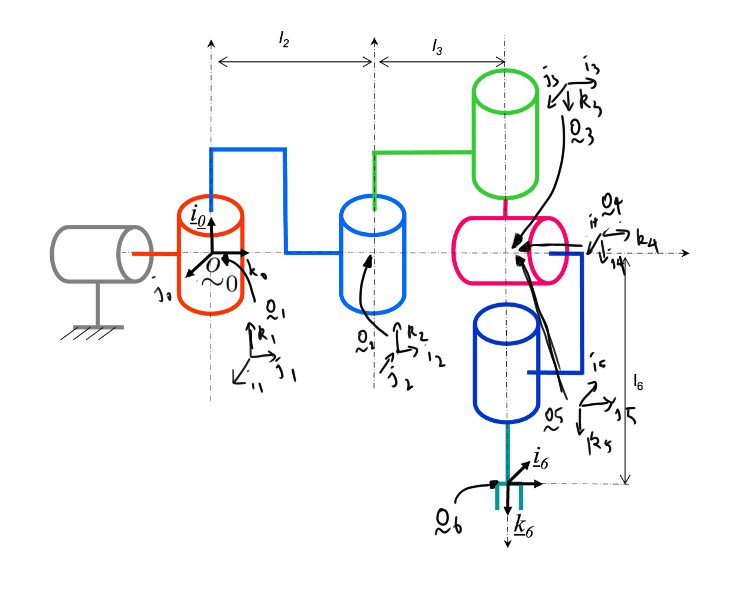
\includegraphics[width=120mm]{imgs/y2025-v1-q2-1.png}
    \end{center}

    \begin{center}
        \begin{tabular}{lllll}
            Link & $\theta$           & $d$   & $a$   & $\alpha$ \\
            1    & $\pi/2 + \theta_1$ & 0     & 0     & $\pi/2$  \\
            2    & $\pi/2+\theta_2$   & 0     & $l_2$ & 0        \\
            3    & $\theta_3$         & 0     & $l_3$ & $\pi$    \\
            4    & $-\pi/2+\theta_4$  & 0     & 0     & $\pi/2$  \\
            5    & $\pi+\theta_5$     & 0     & 0     & $\pi/2$  \\
            6    & $\theta_6$         & $l_6$ & 0     & 0        \\
        \end{tabular}
    \end{center}

    Note link 1 is from gray to red.

    \begin{align*}
        {\,^0T_1} & =
        \begin{bmatrix}
            [e^{\left(\pi/2+\theta_1\right)k\times}] & [0] \\
            [0]                                      & 1
        \end{bmatrix}
        \begin{bmatrix}
            [e^{\left(\pi/2\right)i\times}] & [0] \\
            [0]                             & 1
        \end{bmatrix} \\
                  & =
        \begin{bmatrix}
            [e^{\left(\pi/2+\theta_1\right)k\times} e^{\left(\pi/2\right)i\times}] & [0] \\
            [0]                                                                    & 1
        \end{bmatrix}
    \end{align*}

    \begin{align*}
        {\,^1T_2} & =
        \begin{bmatrix}
            [e^{\left(\pi/2+\theta_2\right)k\times}] & [0] \\
            [0]                                      & 1
        \end{bmatrix}
        \begin{bmatrix}
            [I_3] & [l_2 i] \\
            [0]   & 1
        \end{bmatrix} \\
                  & =
        \begin{bmatrix}
            [e^{\left(\pi/2+\theta_2\right)k\times}] & [l_2 i] \\
            [0]                                      & 1
        \end{bmatrix}
    \end{align*}

    \begin{align*}
        {\,^2T_3} & =
        \begin{bmatrix}
            [e^{\left(\theta_3\right)k\times}] & [0] \\
            [0]                                & 1
        \end{bmatrix}
        \begin{bmatrix}
            [e^{\left(\pi\right)i\times}] & [l_2 i] \\
            [0]                           & 1
        \end{bmatrix} \\
                  & =
        \begin{bmatrix}
            [e^{\left(\theta_3\right)k\times} e^{\left(\pi\right)i\times}] & [e^{\left(\theta_3\right)k\times} l_2 i] \\
            [0]                                                            & 1
        \end{bmatrix}
    \end{align*}

    \begin{align*}
        {\,^3T_4} & =
        \begin{bmatrix}
            [e^{\left(-\pi/2+\theta_4\right)k\times}] & [0] \\
            [0]                                       & 1
        \end{bmatrix}
        \begin{bmatrix}
            [e^{\left(\pi/2\right)i\times}] & [0] \\
            [0]                             & 1
        \end{bmatrix} \\
                  & =
        \begin{bmatrix}
            [e^{\left(-\pi/2+\theta_4\right)k\times} e^{\left(\pi/2\right)i\times}] & [0] \\
            [0]                                                                     & 1
        \end{bmatrix}
    \end{align*}

    \begin{align*}
        {\,^4T_5} & =
        \begin{bmatrix}
            [e^{\left(\pi+\theta_5\right)k\times}] & [0] \\
            [0]                                    & 1
        \end{bmatrix}
        \begin{bmatrix}
            [e^{\left(\pi/2\right)i\times}] & [0] \\
            [0]                             & 1
        \end{bmatrix} \\
                  & =
        \begin{bmatrix}
            [e^{\left(\pi+\theta_5\right)k\times} e^{\left(\pi/2\right)i\times}] & [0] \\
            [0]                                                                  & 1
        \end{bmatrix}
    \end{align*}

    \begin{align*}
        {\,^5T_6} & =
        \begin{bmatrix}
            [e^{\left(\theta_6\right)k\times}] & [l_6k] \\
            [0]                                & 1
        \end{bmatrix}
    \end{align*}
\end{solutionbox}

\begin{solutionbox}[Q2-2]
    \footnotesize
    \begin{align*}
        J & =
        \begin{bmatrix}
            \pv{k}_0\times \left(\ppori{6}-\ppori{0}\right) &
            \pv{k}_1\times \left(\ppori{6}-\ppori{1}\right) &
            \pv{k}_2\times \left(\ppori{6}-\ppori{2}\right) &
            \pv{k}_3\times \left(\ppori{6}-\ppori{3}\right) &
            \pv{k}_4\times \left(\ppori{6}-\ppori{4}\right) &
            \pv{k}_5\times \left(\ppori{6}-\ppori{5}\right)   \\
            \pv{k}_0                                        &
            \pv{k}_1                                        &
            \pv{k}_2                                        &
            \pv{k}_3                                        &
            \pv{k}_4                                        &
            \pv{k}_5
        \end{bmatrix}
    \end{align*}
    \normalsize

    Since $\ppori{3} = \ppori{4}=\ppori{5}$, left multiply with $$$$

    \begin{align*}
        \begin{bmatrix}
            I & \left(\ppori{6}-\ppori{3}\right)\times \\
            0 & I
        \end{bmatrix} J & =
        \begin{bmatrix}
            \pv{k}_0\times \left(\ppori{3}-\ppori{0}\right) &
            \pv{k}_1\times \left(\ppori{3}-\ppori{1}\right) &
            \pv{k}_2\times \left(\ppori{3}-\ppori{2}\right) & 0 & 0 & 0 \\
            \pv{k}_0                                        &
            \pv{k}_1                                        &
            \pv{k}_2                                        &
            \pv{k}_3                                        &
            \pv{k}_4                                        &
            \pv{k}_5
        \end{bmatrix}
    \end{align*}

    Then the system can be analyzed with arm and wrist singularity separately.

    Arm singularity arise when o3 is in the line formed by o0 and k0.

    Wrist singularity when k3 and k5 are inline of $\theta_4=0$

\end{solutionbox}

\begin{solutionbox}[Q2-3]
    Since q0 and q1 can reach point i2 in any direction and the rest can extend l2+l3+l6 away from o0. Then the reachable workspace must have an outer bound of a sphere with radius l2+l3+l6 centered at o0.

    The inner radius of the sphere would be the longest arm minus the two smaller arms and if that is negative, the minimum radius is 0. Expressed mathematically:

    $\max(\max(l2,l3,l6)-(l2+l3+l6 - \max(l2,l3,l6)),0) = \max(2\max(l2,l3,l6)-l2-l3-l6,0)$
\end{solutionbox}

\begin{solutionbox}[Q2-4]
    Due to the spherical wrist, the geometry of the arm and that of the wrist can be analyzed independently.

    There are going to be 8 solutions and I will be referring to them as binaries encoding since they are natural.

    Wrist center is at $\ppori{6}-l6 \pv{k}_6$.

    For o3 to be there, there are four solutions to the arm.

    First project $\ppori{3}-\ppori{0}$ onto the vector $\pv{k}_0$ to get $\left(\ppori{3}-\ppori{0}\right) \parallel \pv{k}_0 = \left(\ppori{3}-\ppori{0}\right) \cdot \pv{k}_0$.

    Then subtract it off from $\ppori{3}-\ppori{0}$ to get  $\left(\ppori{3}-\ppori{0}\right) \perp \pv{k}_0 = \left(\ppori{3}-\ppori{0}\right) - \left(\ppori{3}-\ppori{0}\right) \cdot \pv{k}_0 \pv{k}_0$

    Then use Kahan p1 with $s = j0$ and $t = \left(\ppori{3}-\ppori{0}\right) \perp \pv{k}_0$. Let the result be $\left|\theta_{0-v0}\right|$ This give the absolute value of the angle of $\theta_0$ for half of the solutions.

    The sign of $\theta_{0-v0}$ is the same as $ - \left(\ppori{3}-\ppori{0}\right) \cdot \pv{i}_0$.

    The other version of the solution, $\theta_{0-v0}$ is $\theta_{0-v0}+\pi$

    For each solution, calculate the mean angle for $\theta_2$ which is by removing the component of $\left(\ppori{3}-\ppori{0}\right)$ that is perpendicular to $\pv{k}_1$ and using Kahan P1 between that and $\pv{j}_1$ to find the absolute value of angle to move by. Then use dot product between $\left(\ppori{3}-\ppori{0}\right)$ and $-\pv{i}_1$ to determine the sign. This mean angle changes with which solution is being used for $theta_1$

    The delta from the mean is $\pi - \text{Kahan P4}(a=\left|\ppori{3}-\ppori{0}\right|,b=l_2,c=l_3)$.

    Then, using Kahan p4 with a=l2, b=l3, and c = $\left|\ppori{3}-\ppori{0}\right|$, the absolute value of theta 3 can be found.

    The first solution is then $\theta_2 = \text{mean} + \text{delta}$ and $\theta_3 = -\left|\theta_3\right|$. And the second solution is $\theta_2 = \text{mean} - \text{delta}$ and $\theta_3 = \left|\theta_3\right|$

    Lastly is the wrist orientation. For any given combination of theta 1, 2, and 3, $\ppori{3}$ and $\pc{C}_3$ are set.

    Project k5 onto i3 and j3, calculate the angle formed between $j_3$ and the projection gives $theta_4$. There are two solutions $\pi$ apart.

    Use Kahan p2, u is k3, w is k5, s is k4, solves for theta 4.

    Use Kahan p2, u is i5, w is i6, s is k5 or k6, solves for theta 5.

    % 40 minutes on this alone
\end{solutionbox}


\begin{solutionbox}[Q2-4 alternatively]
    \begin{center}
        \centering
        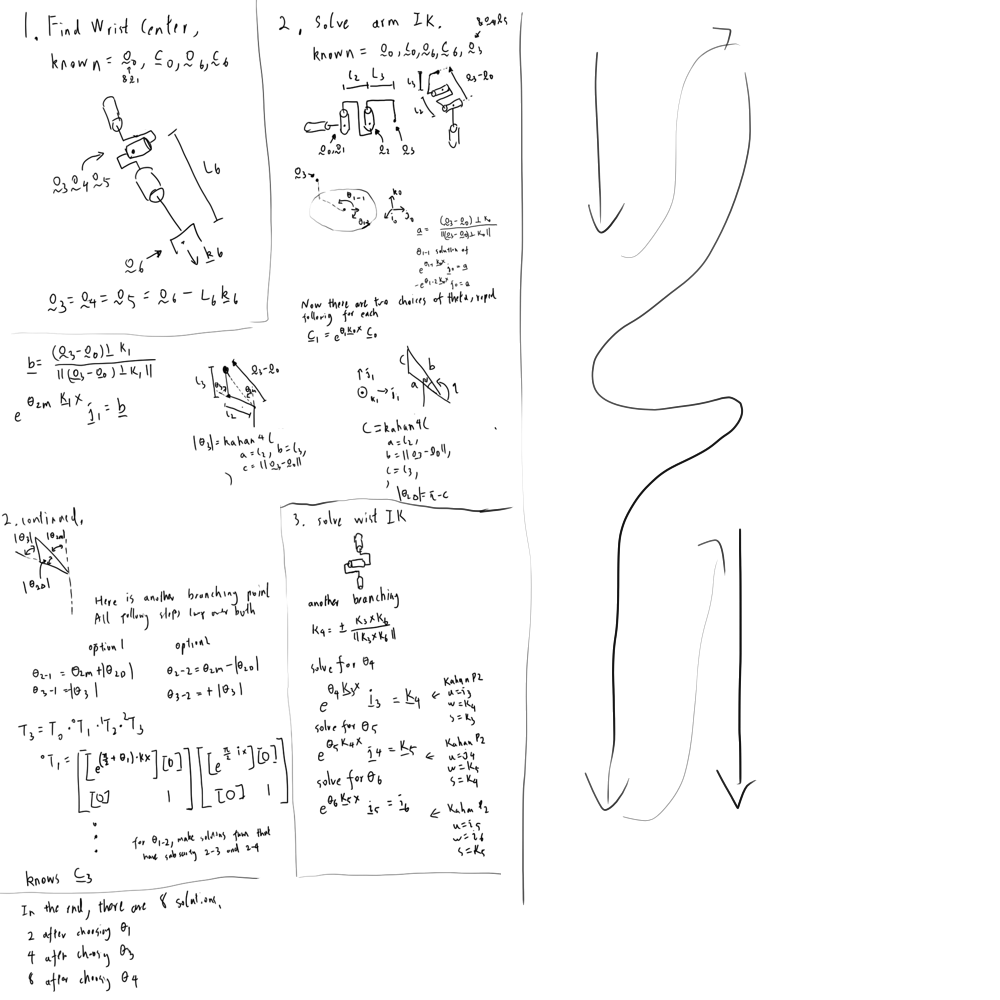
\includegraphics[width=\textwidth]{imgs/y2025-v1-q2-4.png}
    \end{center}
\end{solutionbox}

\begin{solutionbox}[Q2-4?]
    This is a task space stiffness controller.


    \begin{align*}
        {^0\delta_x} = x_r-x              \\
        {\,^0F} = {\,^0K_p}{\,^0\delta x} \\
        \tau=J^T {\,^0F}                  \\
    \end{align*}

    \begin{align*}
        {^0\delta_x} = x_r-x                     \\
        {\,^s\delta x} ={\,^sC_0} {\,^0\delta x} \\
        {\,^sF} = {\,^sK_p}{\,^s\delta x}        \\
        {\,^0F} = {\,^0C_s}{\,^sF}               \\
        \tau=J^T {\,^0F}                         \\
    \end{align*}

    % 4:15
\end{solutionbox}
